\documentclass{article}

\usepackage[english]{babel}
\usepackage[utf8]{inputenc}
\usepackage{amsmath,amssymb}
\usepackage{parskip}
\usepackage{graphicx}
\usepackage{hyperref}

% Margins
\usepackage[top=2.5cm, left=3cm, right=3cm, bottom=4.0cm]{geometry}
% Colour table cells
\usepackage[table]{xcolor}

% Red box around equation
\usepackage[skins, theorems]{tcolorbox}
\tcbset{highlight math style={enhanced, colframe=red,colback=white,arc=0pt,boxrule=1pt}}

% Code listing with highlight
\usepackage{listings}
\definecolor{codegreen}{rgb}{0,0.6,0}
\definecolor{codegray}{rgb}{0.5,0.5,0.5}
\definecolor{codepurple}{rgb}{0.58,0,0.82}
\definecolor{backcolour}{rgb}{0.95,0.95,0.92}

\lstdefinestyle{style1}{
    backgroundcolor=\color{backcolour},
    commentstyle=\color{codegreen},
    keywordstyle=\color{magenta},
    numberstyle=\tiny\color{codegray},
    stringstyle=\color{codepurple},
    basicstyle=\ttfamily,
    breakatwhitespace=false,
    breaklines=true,
    postbreak=\mbox{\textcolor{red}{$\hookrightarrow$}\space},
    captionpos=b,
    keepspaces=true,
    numbers=left,
    numbersep=5pt,
    showspaces=false,
    showstringspaces=false,
    showtabs=false,
    tabsize=4,
    frame=lines,
    language=Python,
    columns=fullflexible,
}

\lstset{style=style1}

% Get larger line spacing in table
\newcommand{\tablespace}{\\[1.25mm]}
\newcommand\Tstrut{\rule{0pt}{2.6ex}}         % = `top' strut
\newcommand\tstrut{\rule{0pt}{2.0ex}}         % = `top' strut
\newcommand\Bstrut{\rule[-0.9ex]{0pt}{0pt}}   % = `bottom' strut

%%%%%%%%%%%%%%%%%
%     Title     %
%%%%%%%%%%%%%%%%%
\title{16824 Homework 3}
\author{Jiajun Wan \\ Andrew ID: jiajunw2}
\date{}

\begin{document}
\maketitle

\setcounter{section}{1}
\section*{Task 1: Understanding VQA}

\setcounter{subsection}{0}
\subsection{Why do you think that it's computationally costly to use all answers as separate classes instead of keeping only the most frequent ones?}
We have to use a large number of output neurons, that add computations on final sigmoid/softmax calculation, loss computation, and backward propagation. Keeping only the most frequent ones will largely reduce the amount of calculations.

\subsection{Complete the \_\_init\_\_ method of the dataset class for VQA in vqa\_dataset.py. Specifically, initialize the VQA API and anything you need from that.}
\begin{lstlisting}
self._vqa = VQA(annotation_file=annotation_json_file_path,
                question_file=question_json_file_path)
\end{lstlisting}

\subsection{Implement the \_\_len\_\_ method of the VQADataset class. Should the size of the dataset be equal to the number of images, questions or the answers?}
\begin{lstlisting}
def __len__(self):
    # total number of questions
    return len(self._vqa.qqa)
\end{lstlisting}
The size of the dataset be equal to the number of questions.

\subsection{Complete the \_\_getitem\_\_ method}
\begin{lstlisting}
q_anno = self._vqa.qa[idx]  # load annotation
q_str = self._vqa.qqa[idx]['question']  # question in str format
\end{lstlisting}
\newpage

\setcounter{section}{2}
\section*{Task 2: Building a pipeline for VQA}

\setcounter{subsection}{0}
\subsection{What should be the output dimension of the trainable linear layer? Complete the corresponding part in the \_\_init\_\_ method of BaselineNet in models.py.}
\begin{lstlisting}
self.classifier = nn.Linear(
    self.text_encoder.config.hidden_size + 512,
    n_answers,
)
\end{lstlisting}
It should be n\_answers (5127)

\subsection{Implement compute\_vis\_feats that featurizes the image (it can be implemented as an one-liner!).}
\begin{lstlisting}
def compute_vis_feats(self, image):
    """Convert image tensors to feature tensors."""
    return torch.nn.functional.adaptive_avg_pool2d(self.vis_encoder(image), 1).squeeze() # feed to vis_encoder and then mean pool on spatial dims
\end{lstlisting}

\subsection{Implement the forward pass of BaselineNet. Make sure to use compute\_vis\_feats and compute\_text\_feats.}
\begin{lstlisting}
def forward(self, image, question):
    """Forward pass, image (B, 3, 224, 224), qs list of str."""
    text_feats = self.compute_text_feats(question)
    vis_feats = self.compute_vis_feats(image)
    concate_feats = torch.hstack((text_feats, vis_feats))
    logits = self.classifier(concate_feats)
    return logits
\end{lstlisting}

\subsection{What is the loss for multi-label classification? (Hint: in HW1 you also tackled a multi-class classification problem)}
Binary Cross-Entropy Loss

\subsection{Implement the loss call and the optimization code in the train\_test\_loop method.}
\begin{lstlisting}
loss = F.binary_cross_entropy_with_logits(scores, answers)

# Update
if mode == 'train':
    # optimize loss
    loss.backward()
    self.optimizer.step()
    self.optimizer.zero_grad()
\end{lstlisting}

\subsection{Complete the train\_test\_loop method to monitor the performance in Tensorboard. Plot the loss and accuracy and include these in your report. Additionally show multiple image-question pairs (at least 3) with the respective answers (predicted and ground-truth).}
\begin{lstlisting}
    # add code to show the question
    self.writer.add_text(
        'Question%d' % i, data['question'][i],
        epoch * _n_show + i
    )
    # the gt answer
    self.writer.add_text(
        'GT Answer%d' % i, self._id2answer[(data['answers'][i] == 1).nonzero(as_tuple=True)[0][0].item()],
        epoch * _n_show + i
    )
    # and the predicted answer
    self.writer.add_text(
        'Predicted Answer%d' % i, self._id2answer[scores.argmax(1)[i].item()],
        epoch * _n_show + i
    )
# add code to plot the current accuracy
self.writer.add_scalar(
'Acc/' + mode, n_correct / n_samples,
epoch * len(self.data_loaders[mode]) + step
)
\end{lstlisting}
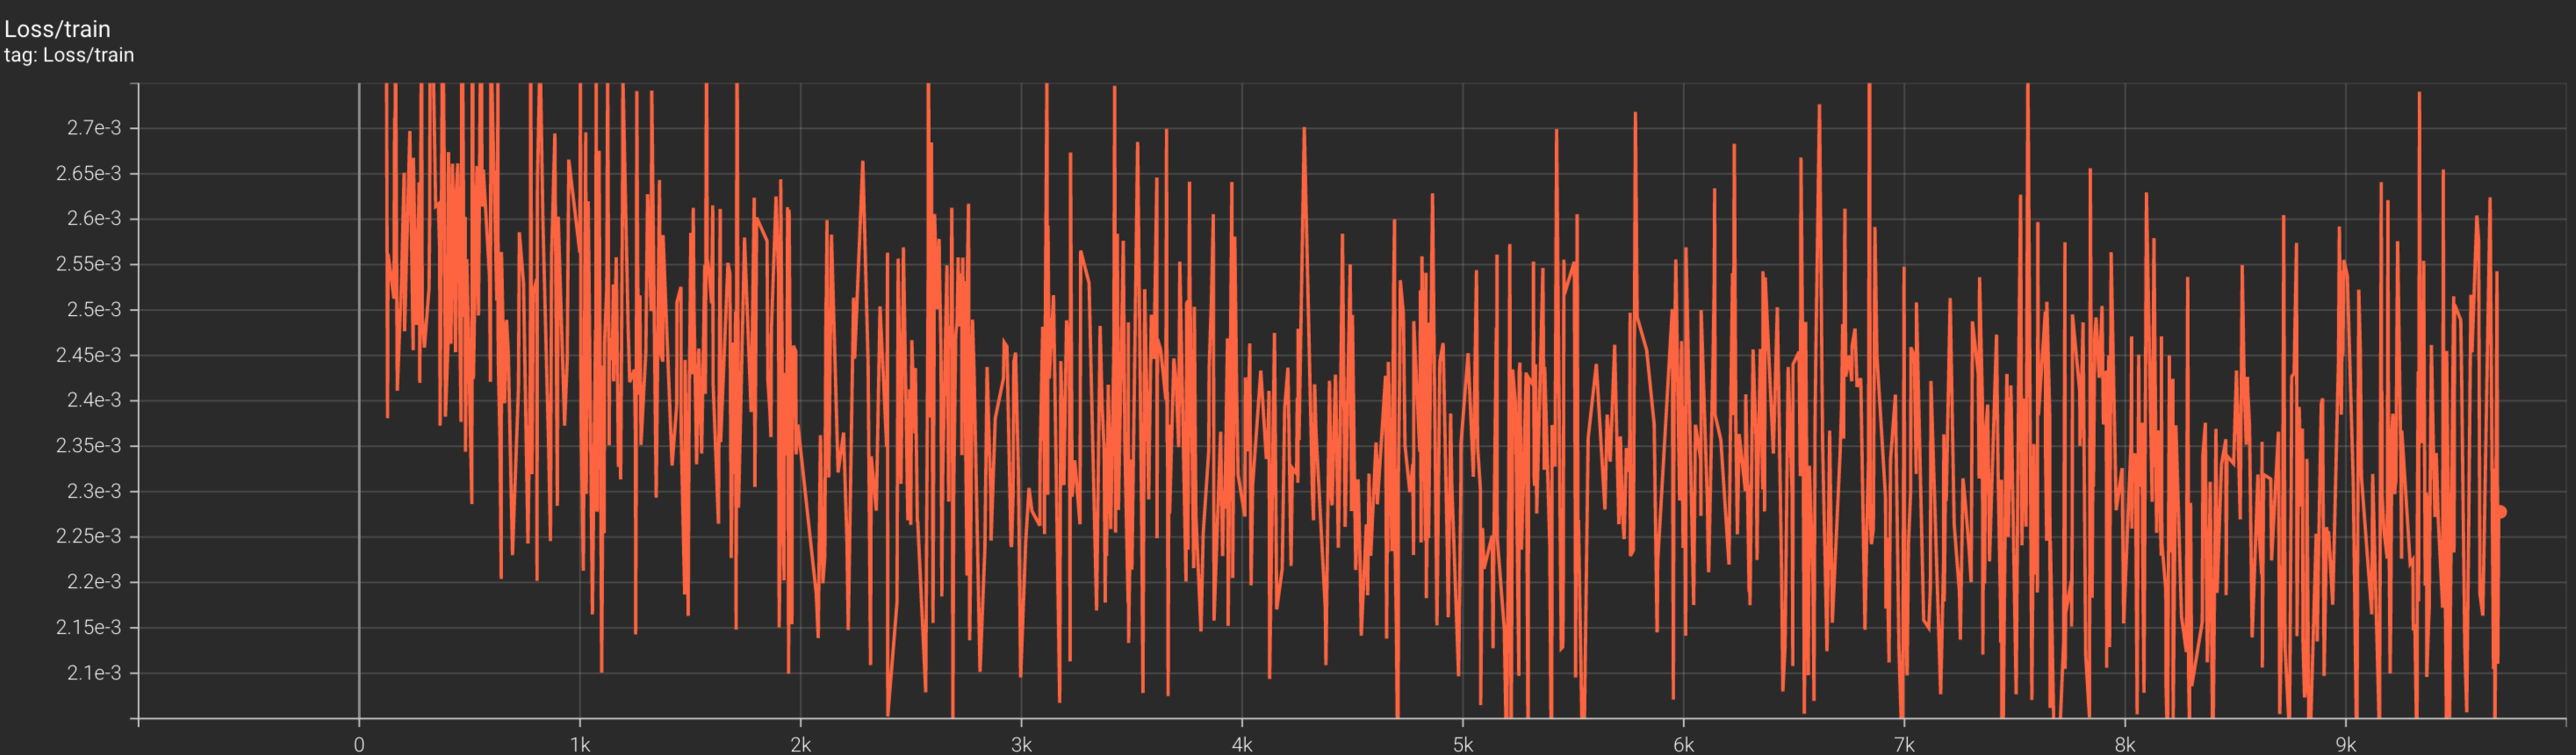
\includegraphics[width=\textwidth]{q2.6_1.png}
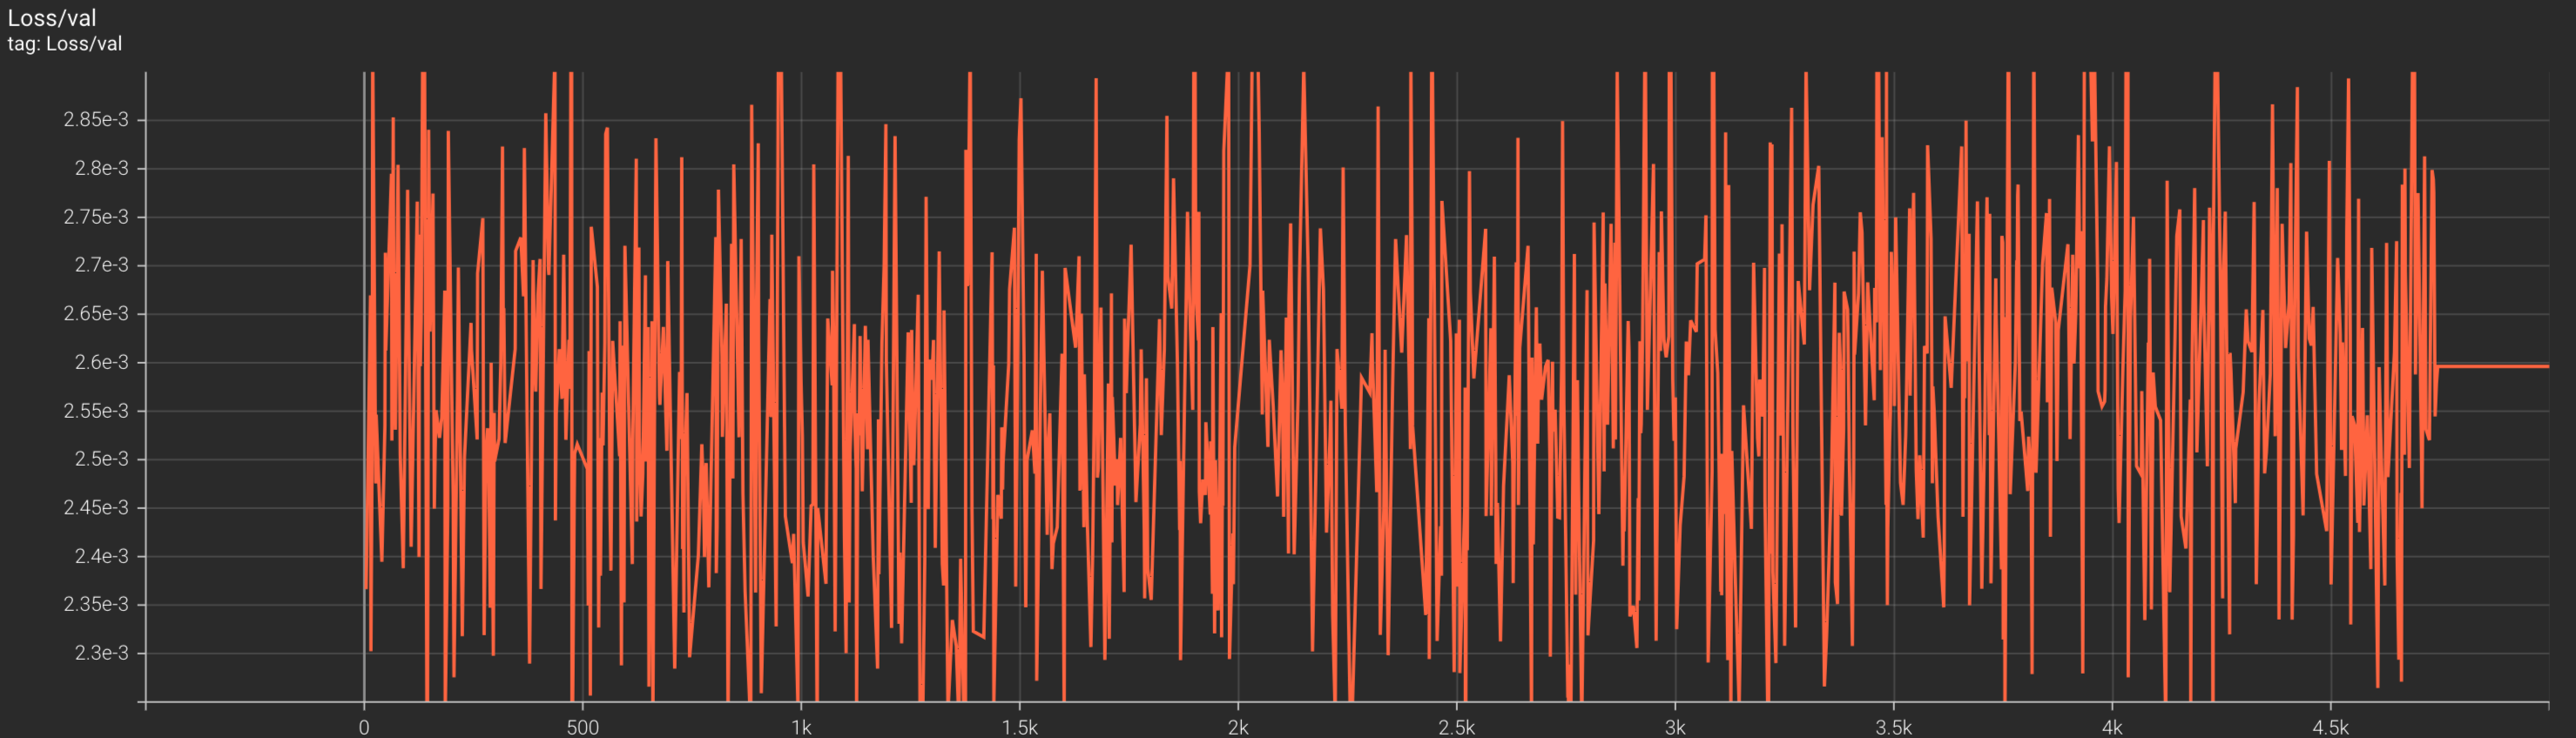
\includegraphics[width=\textwidth]{q2.6_2.png}
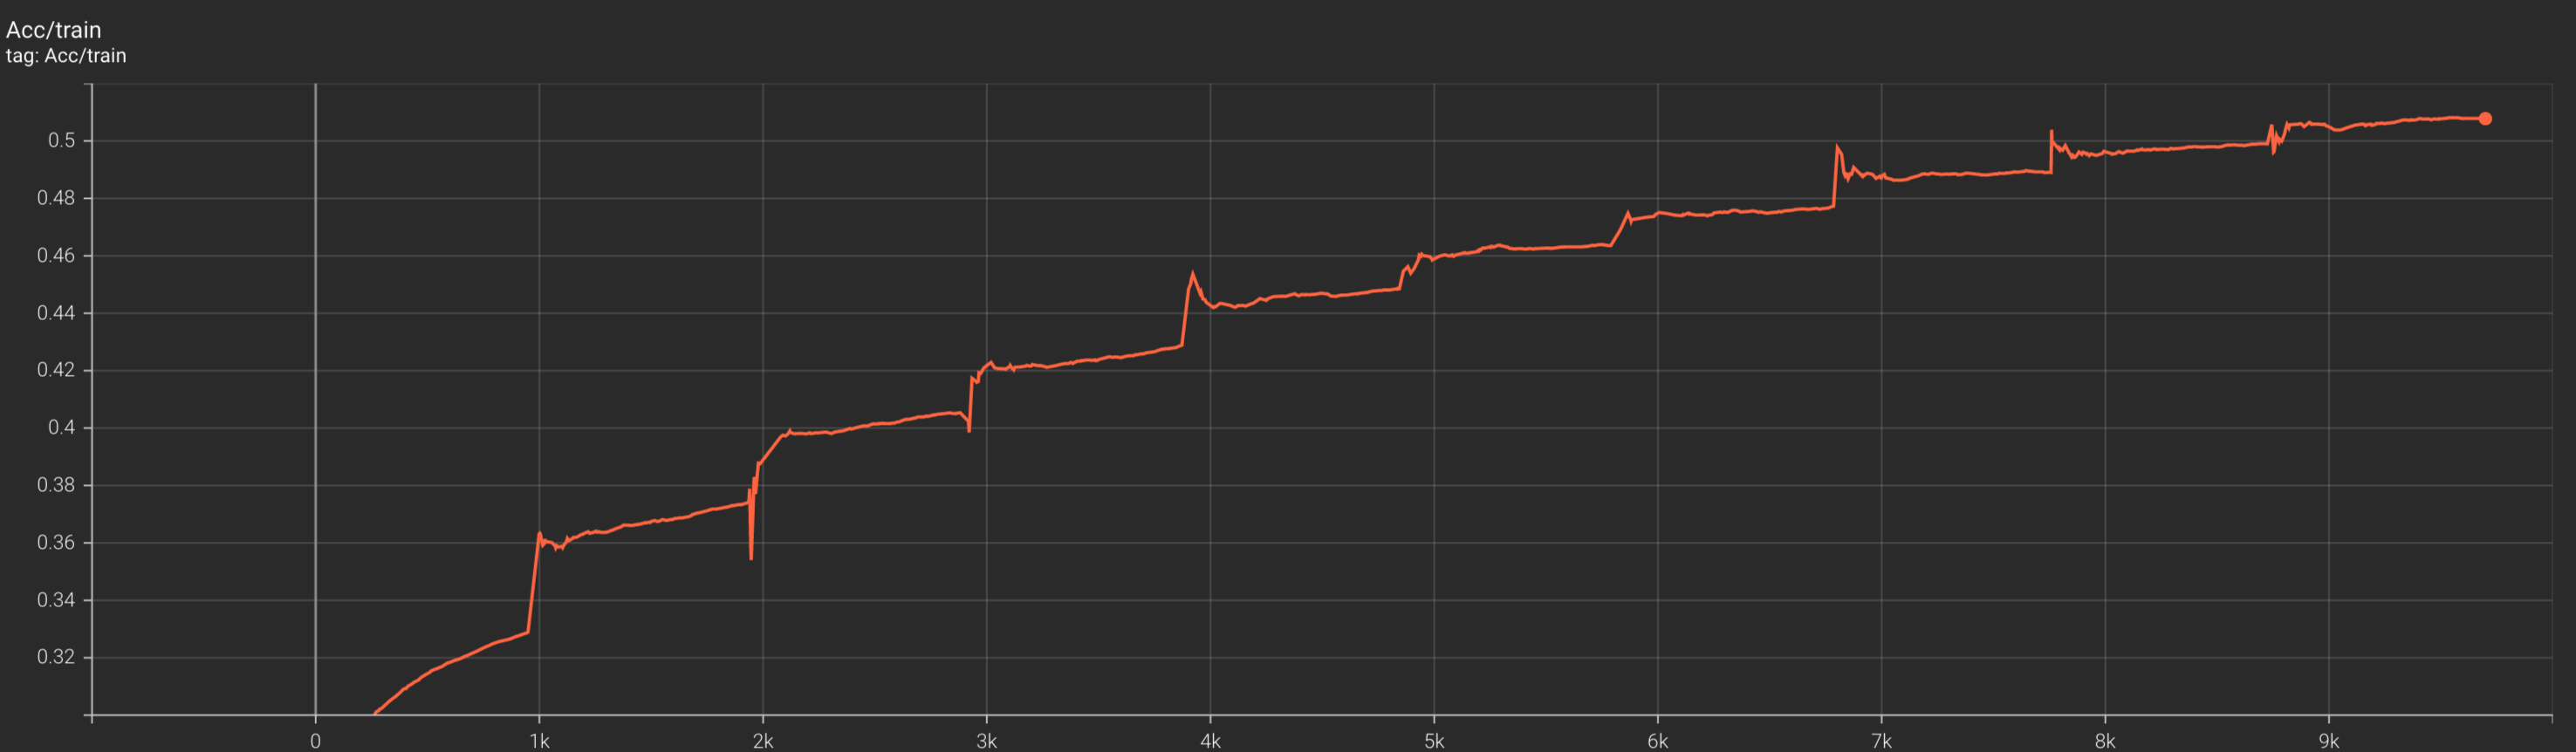
\includegraphics[width=\textwidth]{q2.6_3.png}
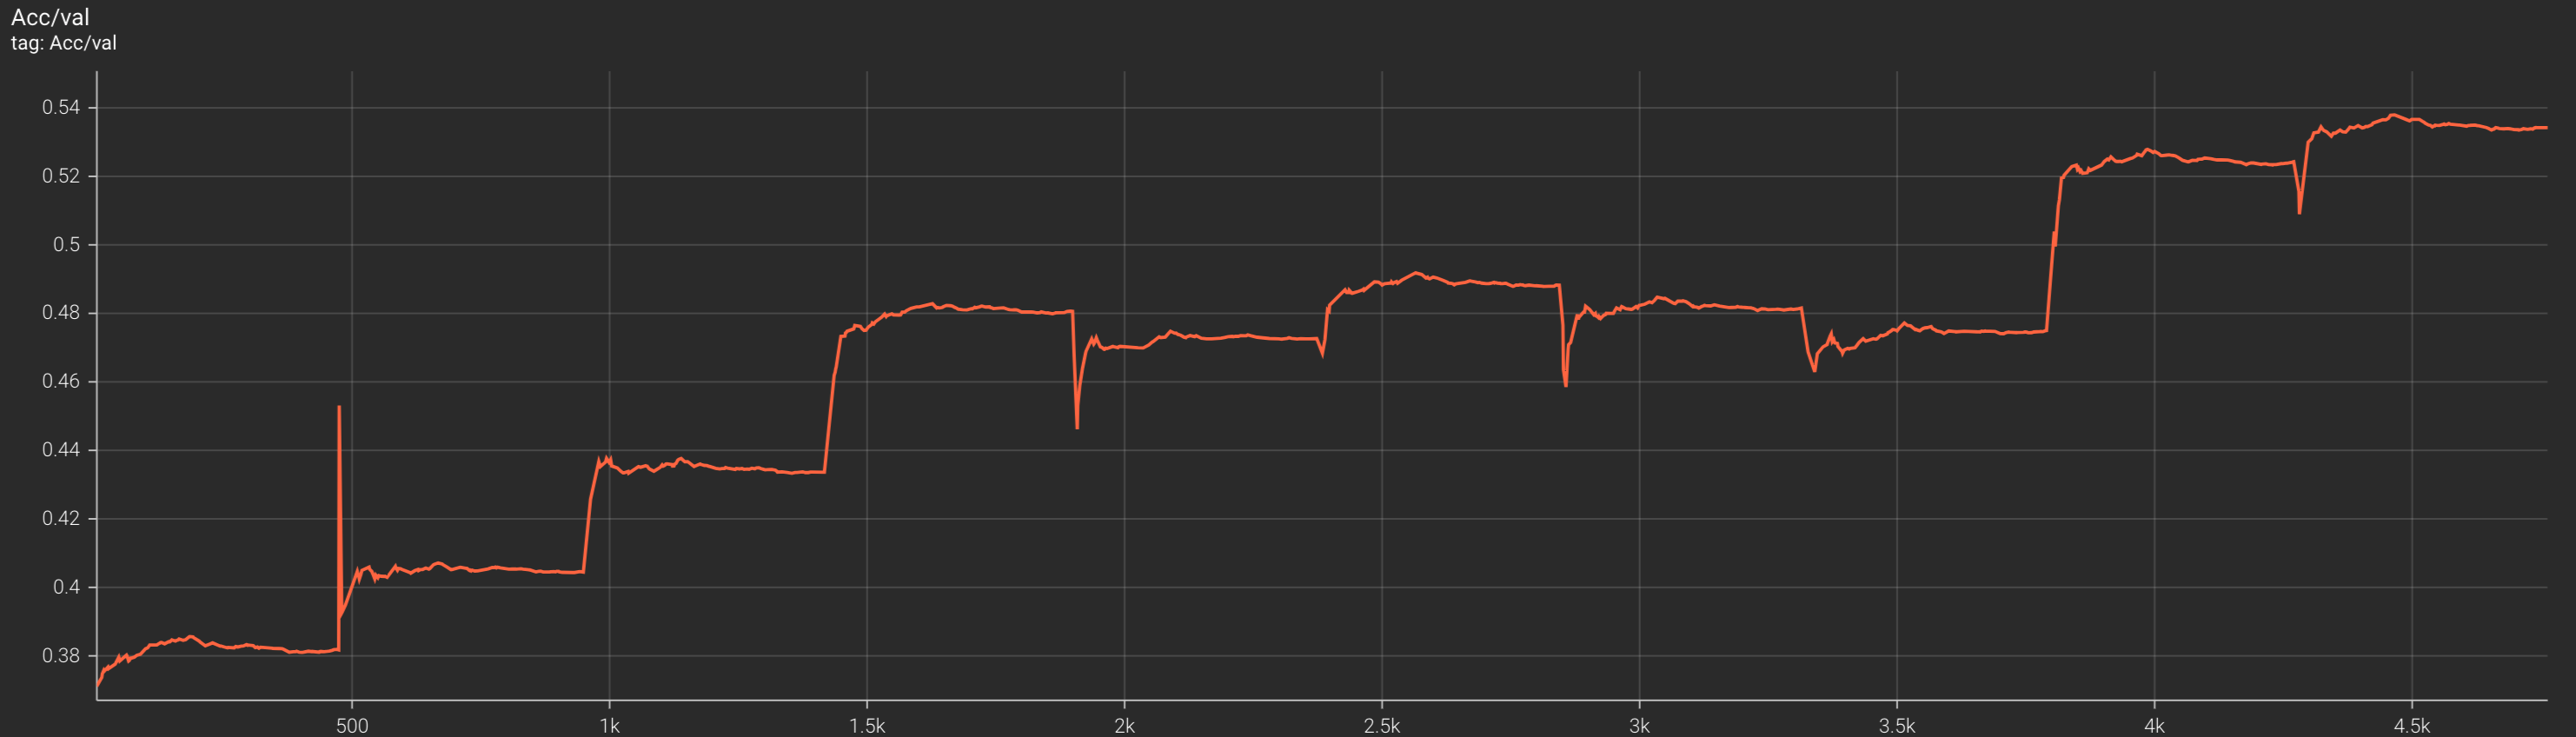
\includegraphics[width=\textwidth]{q2.6_4.png}
\begin{tabular}{ccc}
    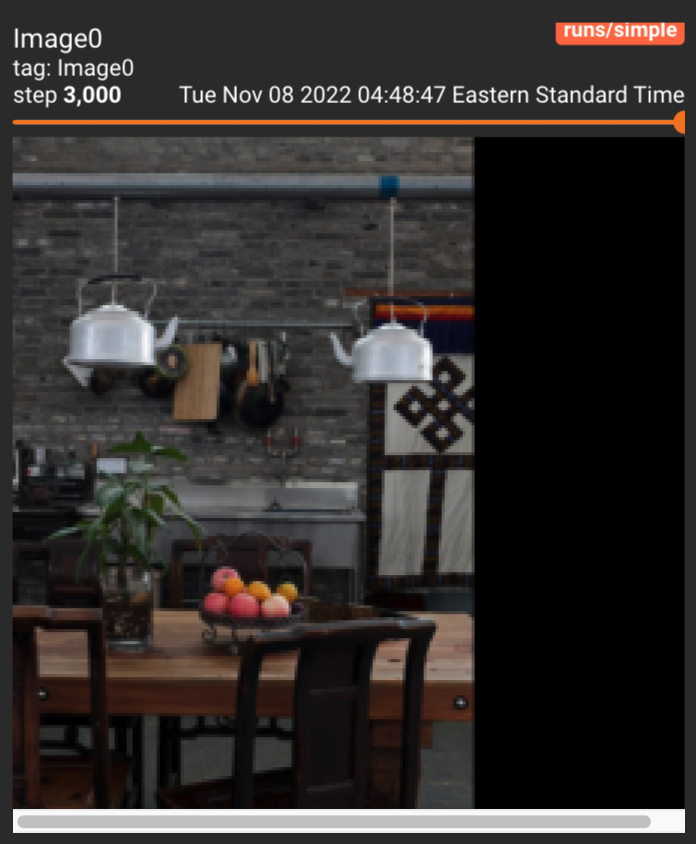
\includegraphics[width=0.33\textwidth]{q2.6_5.png} &
    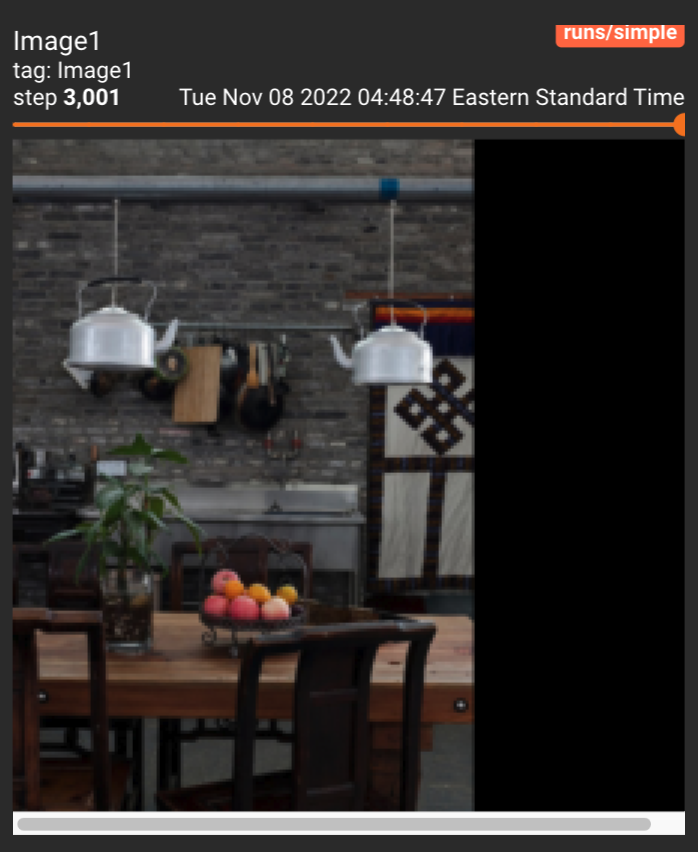
\includegraphics[width=0.33\textwidth]{q2.6_6.png} &
    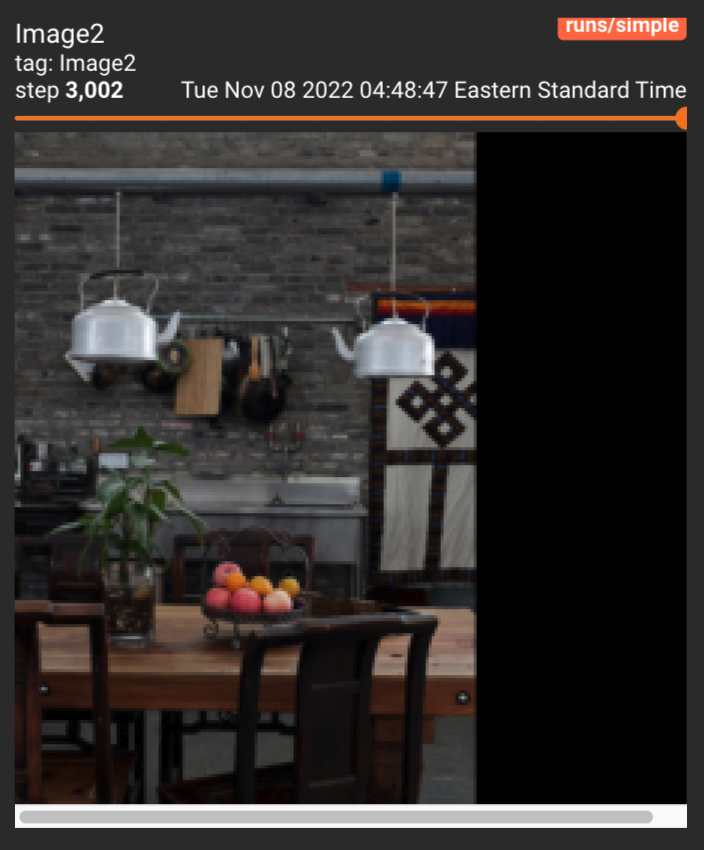
\includegraphics[width=0.33\textwidth]{q2.6_7.png} \\
    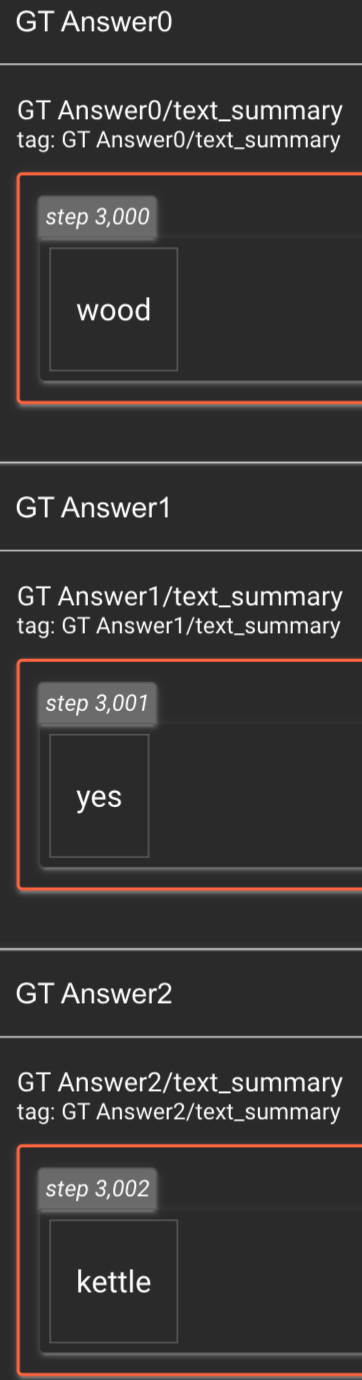
\includegraphics[width=0.3\textwidth]{q2.6_8.png} &
    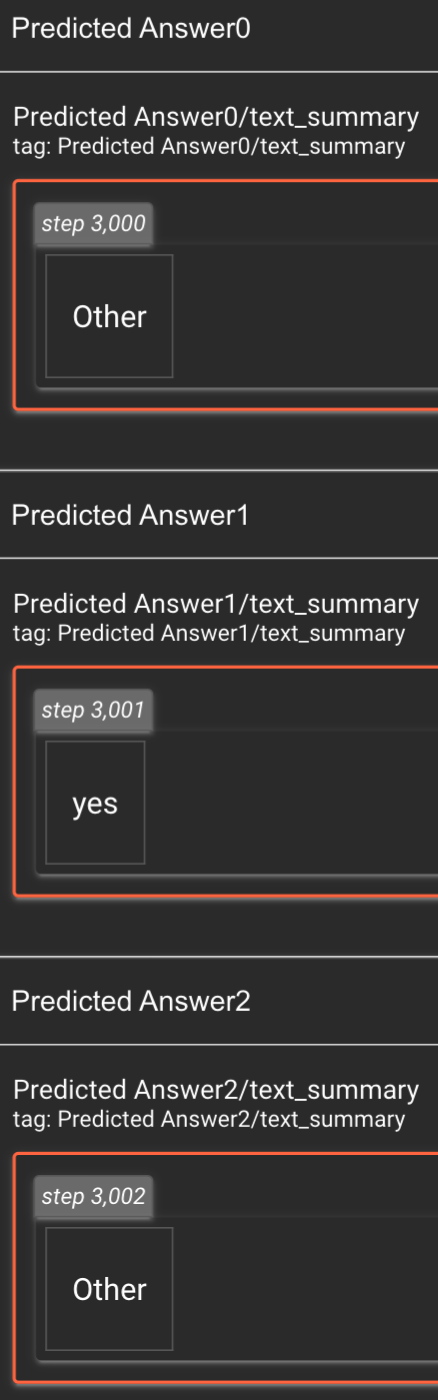
\includegraphics[width=0.3\textwidth]{q2.6_9.png} &
    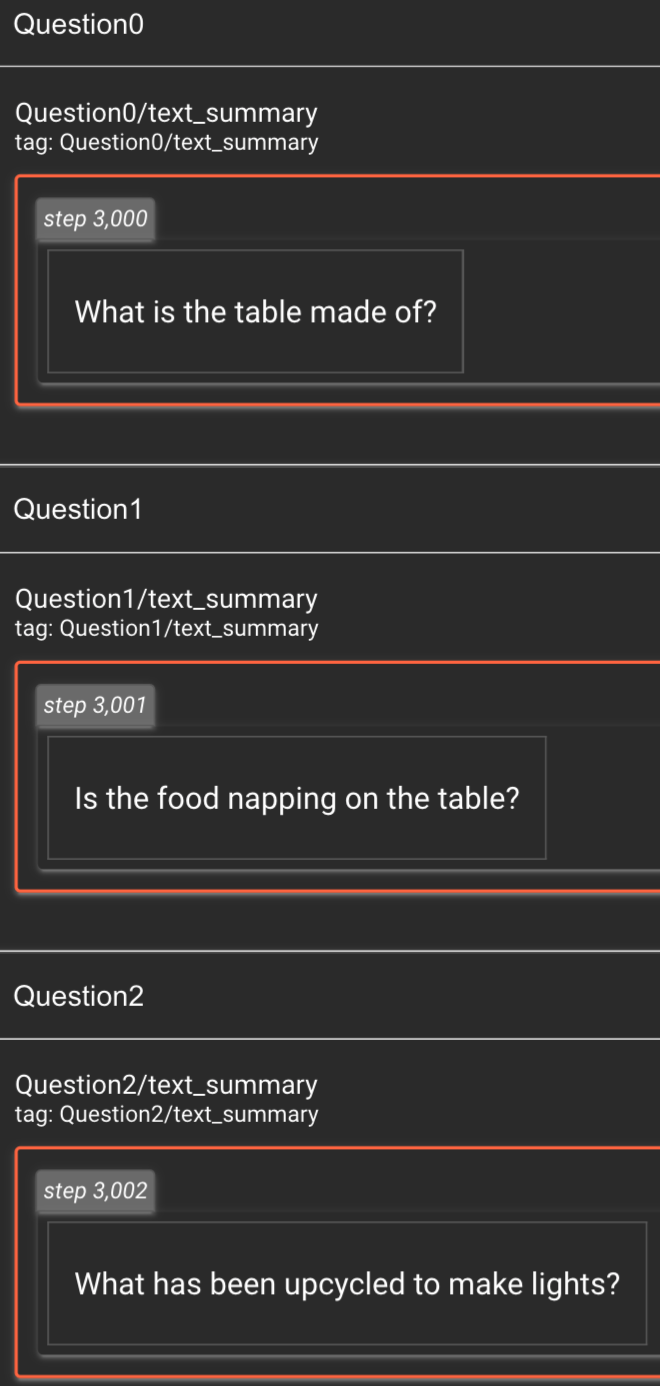
\includegraphics[width=0.3\textwidth]{q2.6_10.png} \\
\end{tabular}
\begin{tabular}{ccc}
    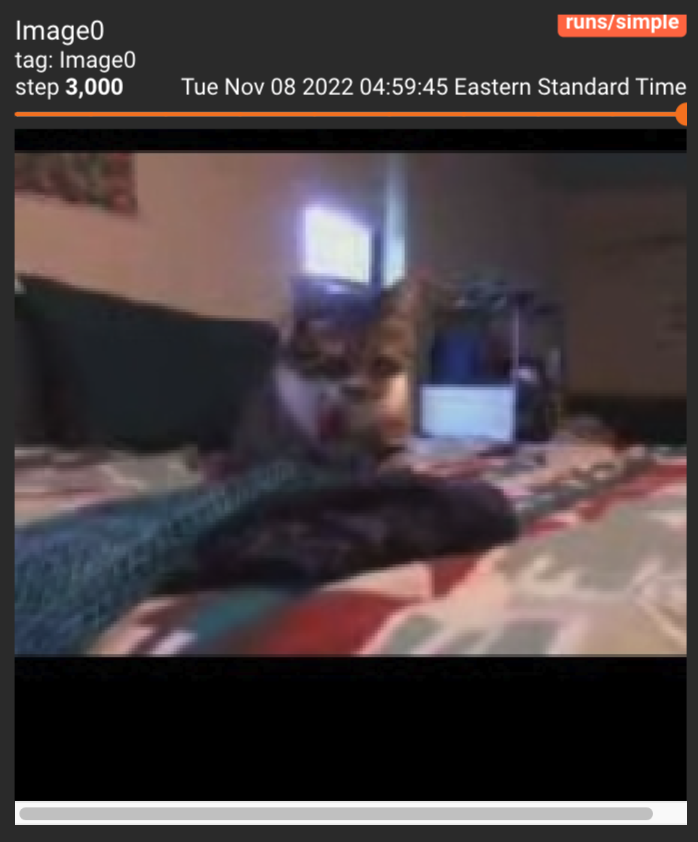
\includegraphics[width=0.33\textwidth]{q2.6_11.png} &
    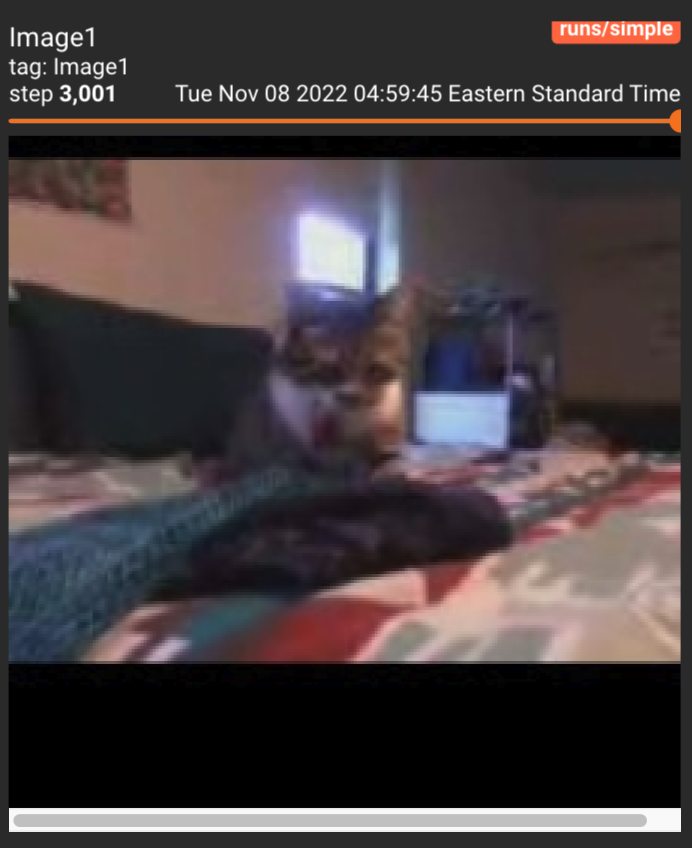
\includegraphics[width=0.33\textwidth]{q2.6_12.png} &
    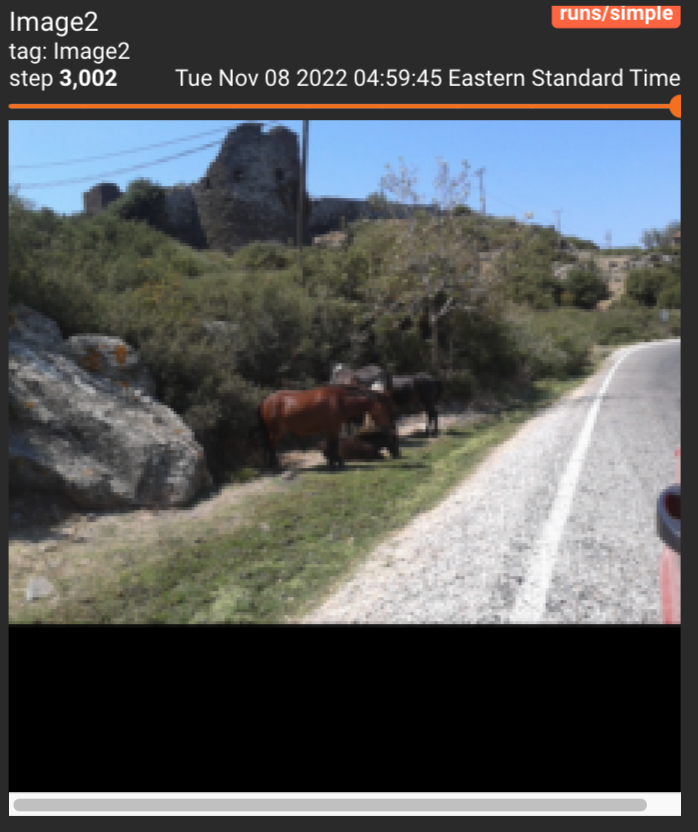
\includegraphics[width=0.33\textwidth]{q2.6_13.png} \\
    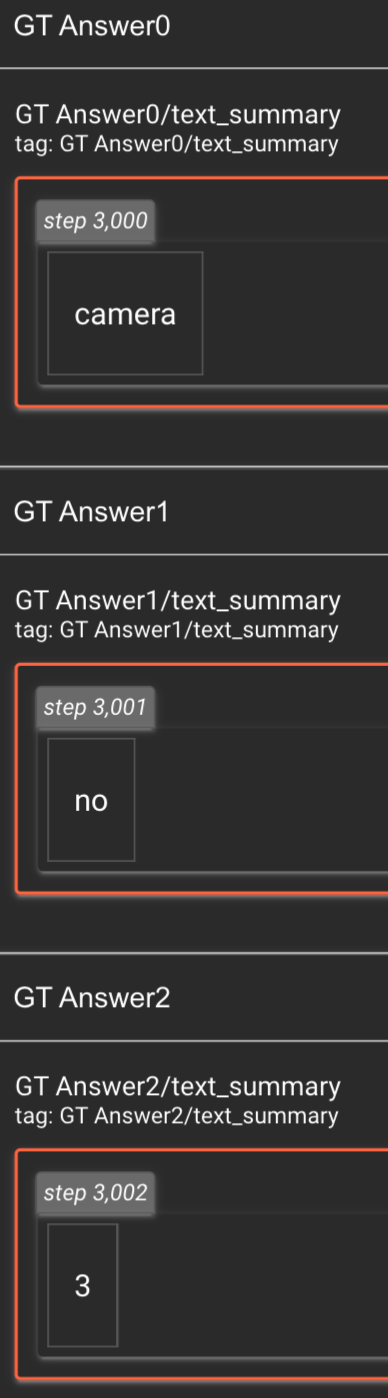
\includegraphics[width=0.3\textwidth]{q2.6_14.png} &
    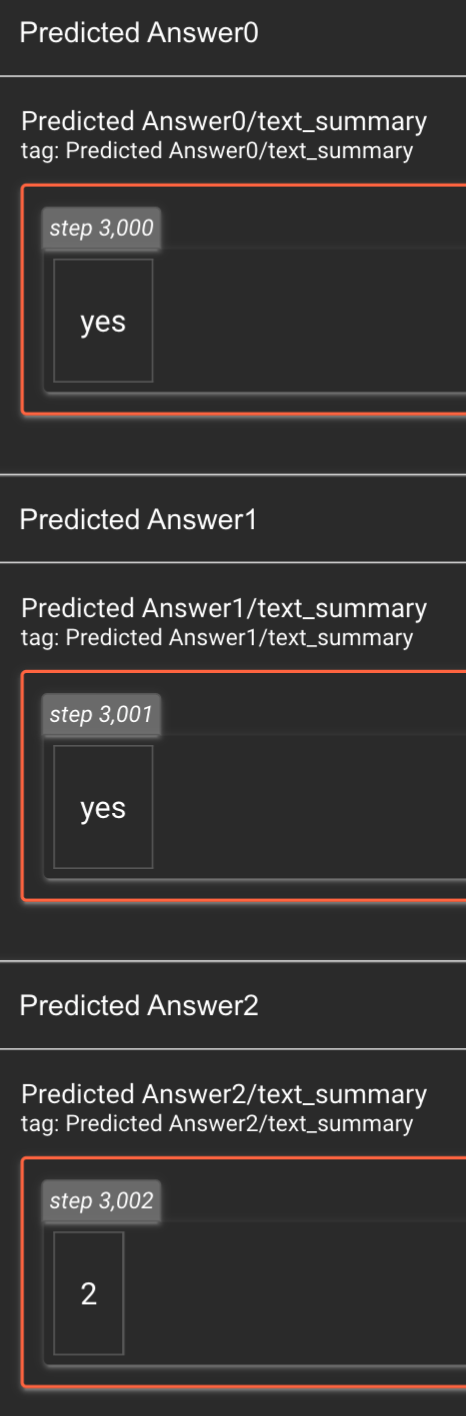
\includegraphics[width=0.3\textwidth]{q2.6_15.png} &
    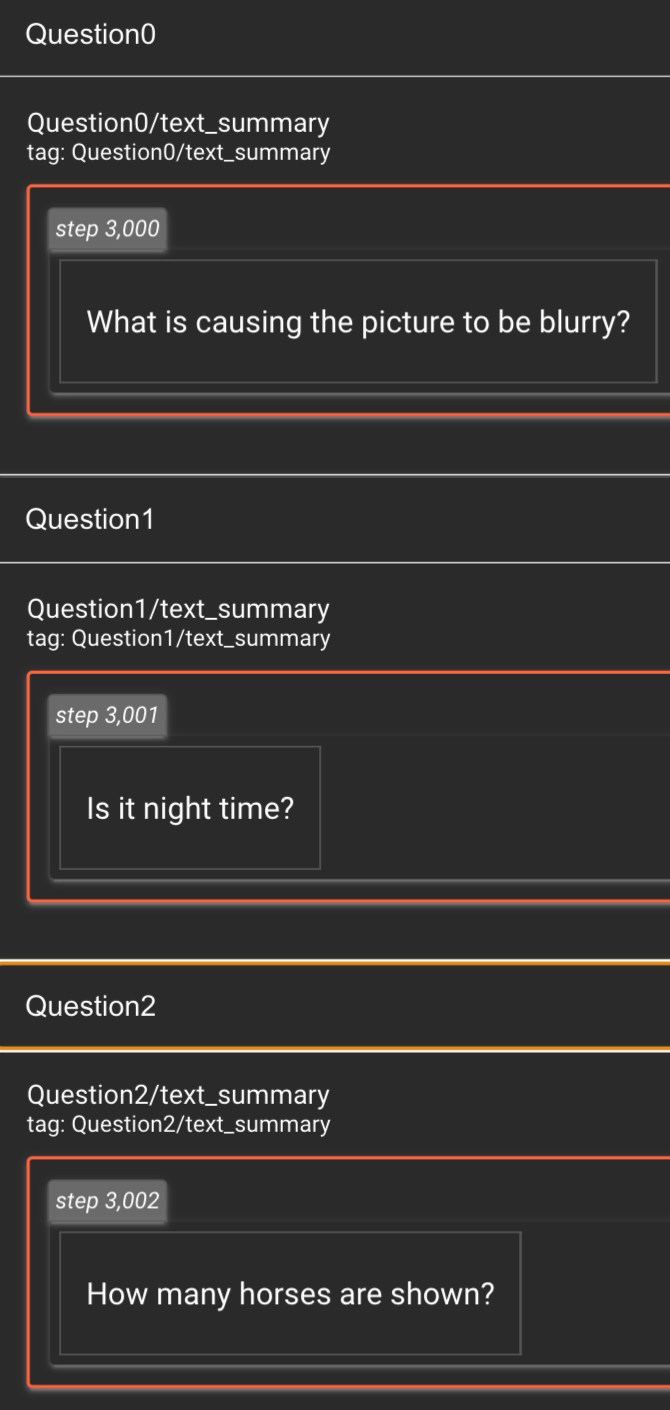
\includegraphics[width=0.3\textwidth]{q2.6_16.png} \\
\end{tabular}
\begin{tabular}{ccc}
    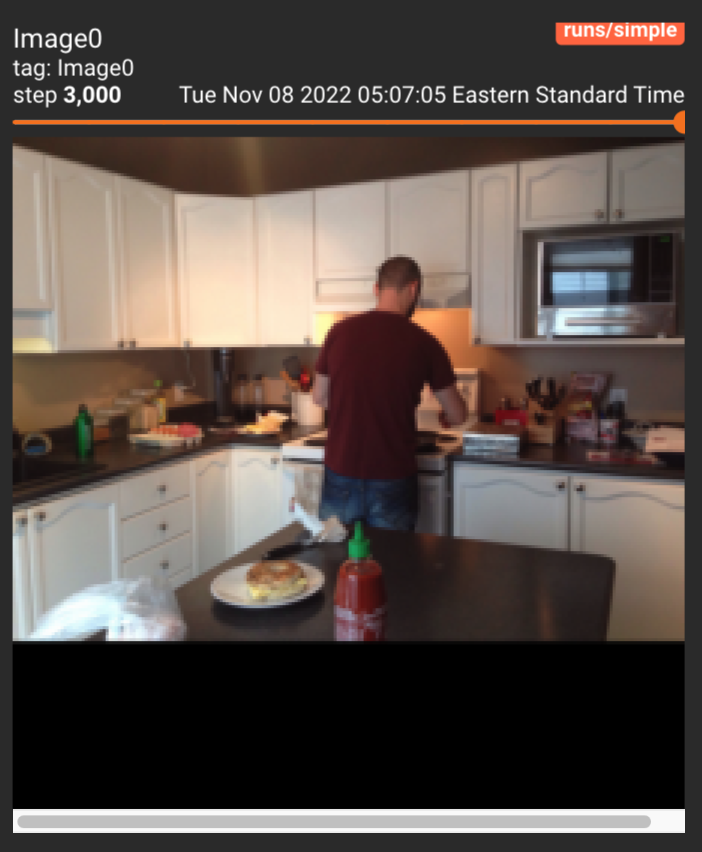
\includegraphics[width=0.33\textwidth]{q2.6_17.png} &
    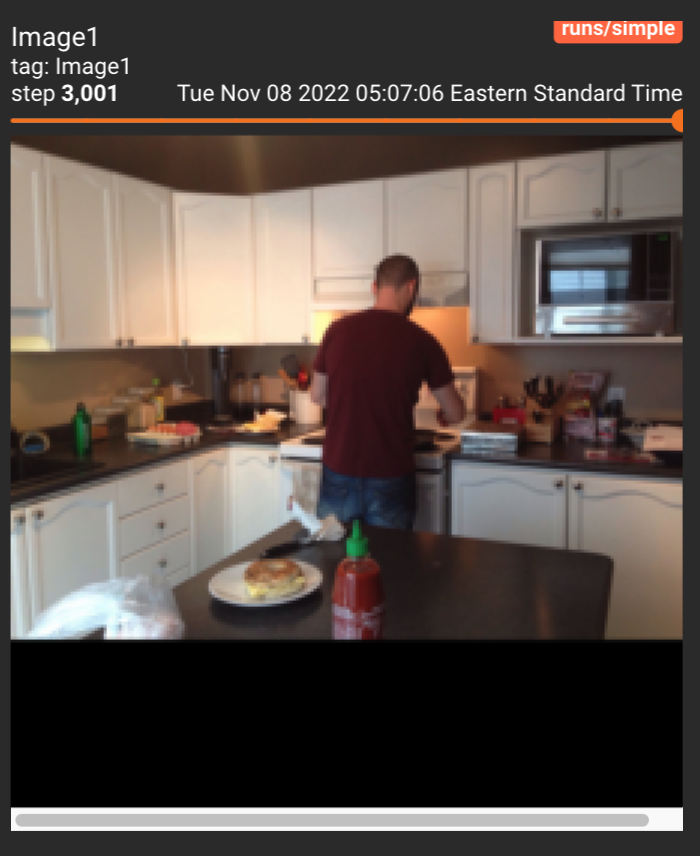
\includegraphics[width=0.33\textwidth]{q2.6_18.png} &
    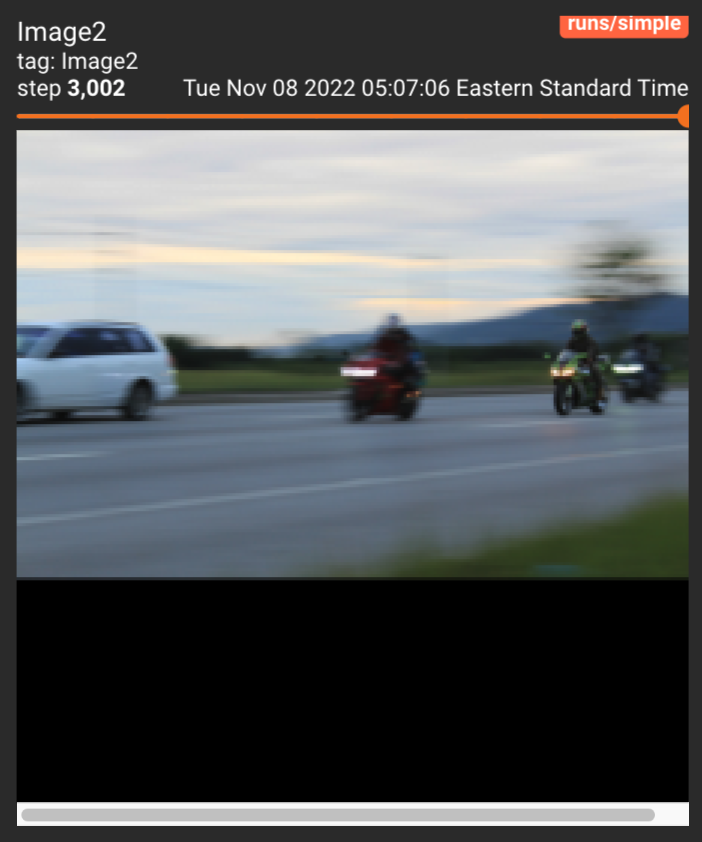
\includegraphics[width=0.33\textwidth]{q2.6_19.png} \\
    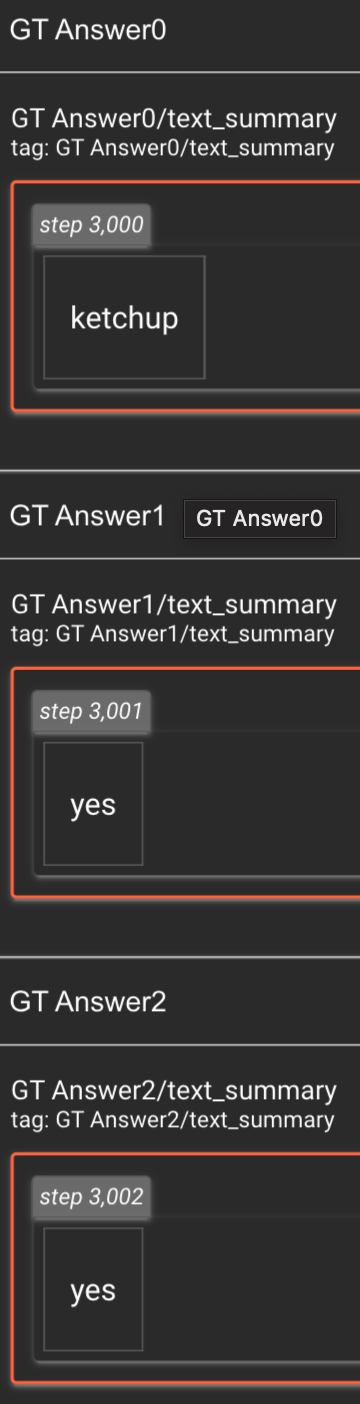
\includegraphics[width=0.3\textwidth]{q2.6_20.png} &
    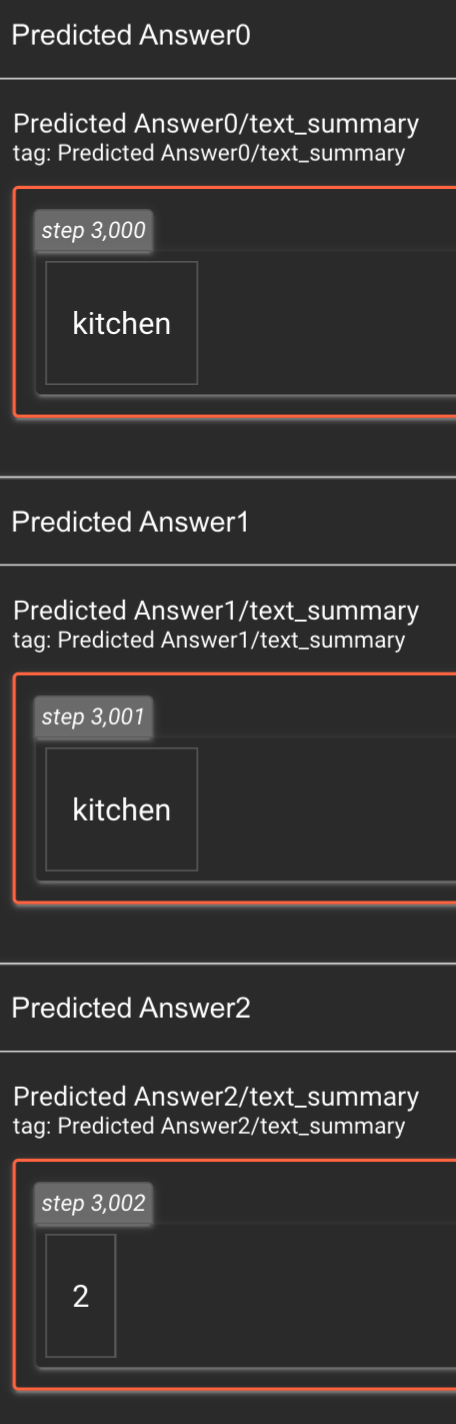
\includegraphics[width=0.3\textwidth]{q2.6_21.png} &
    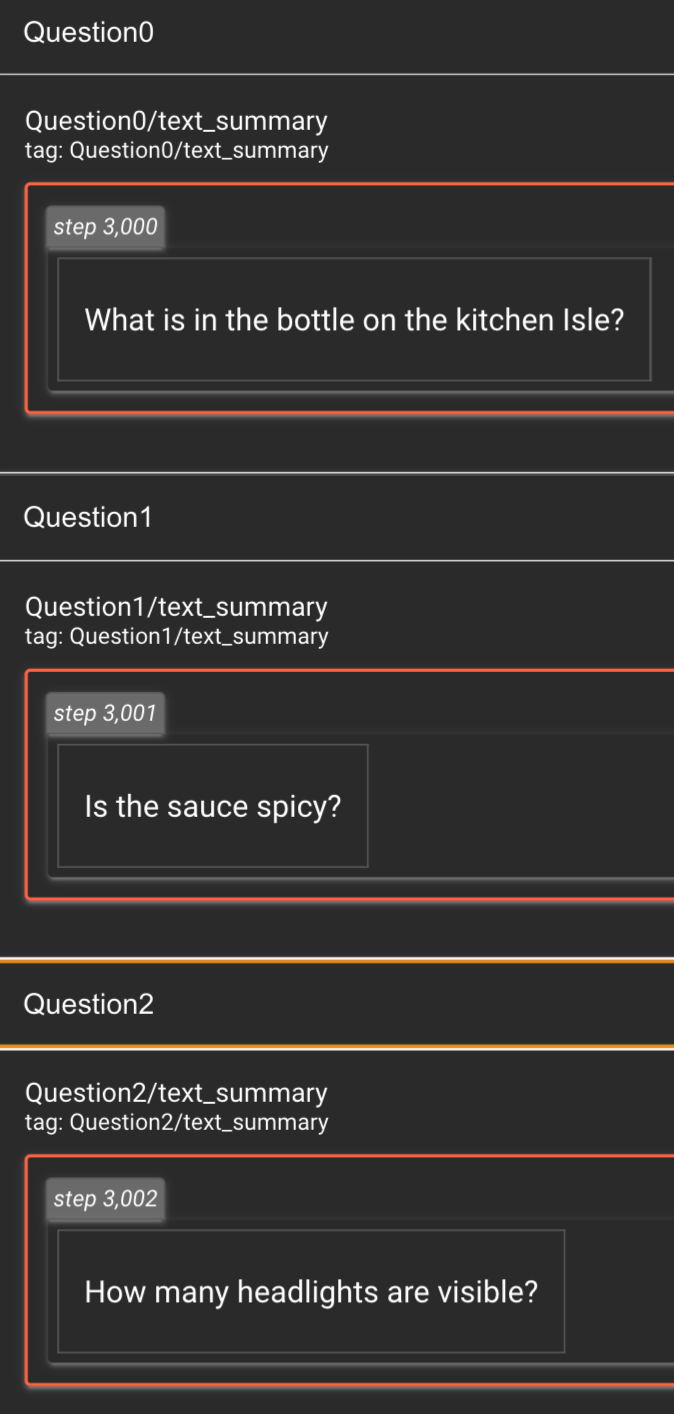
\includegraphics[width=0.3\textwidth]{q2.6_22.png} \\
\end{tabular}

Final Val Acc: 0.5341694647442228

\end{document}